\chapter{Vergleich der Browser}
\label{chapter:vergleich-der-browser}

In diesem Kapitel werden die untersuchten Browser hinsichtlich ihrer hinterlassenen PB Artefakte verglichen.

\subsection*{Common Locations}
Bei keinem Browser konnten PB Artefakte über die Analyse der Datei-Schreiboperationen in den Process Monitor Logfiles gefunden werden.
Ebenso konnten durch die genaue Untersuchung der Entwicklung der SQLite-Datenbänke aller Browser keine PB Artefakte identifiziert werden.
Somit sind die Common Locations aller Browser während der gesamten Versuchsdurchführung frei von PB Artefakten

\subsection*{Registry}
Bei Betrachtung der Registry als Common Locations wurden keine PB Artefakte in den Registry-Key bzw. -Values der Registry-Schreiboperationen der Process Monitor Logfiles gefunden.
Unter Betrachtung der Registry als Uncommon Locations konnten weder in System- noch User-Hives PB Artefakte gefunden werden.
Somit befinden sich bei jedem Browser auch in der Registry zu keinem Zeitpunkt PB Artefakte.

\subsection*{Uncommon Locations}
Weder über Autopsy Stichwortsuche noch in den automatisch von Autopsy kategorisierten Dateien konnten für keinen Browser PB Artefakte identifiziert werden.
%evtl. unterschiedlich Kategorisierte Dateien hervorheben

Einzig über die Untersuchung der Arbeitsspeicherabbilder mit Volatility konnten PB Artefakte zu unterschiedlichen Zeitpunkten der Versuchsdurchführung identifiziert werden. 
Wie in Abbildung \ref{chart:all-browsers-ram-summary} dargestellt, konnten in keinem der Browser vor Durchführung des Browsing Szenarios (RAM-Dump 1) PB Artefakte im Arbeitsspeicher gefunden werden.
\begin{table}[h!]
	\resizebox{\linewidth}{!}{
	\begin{tabular}{r}
		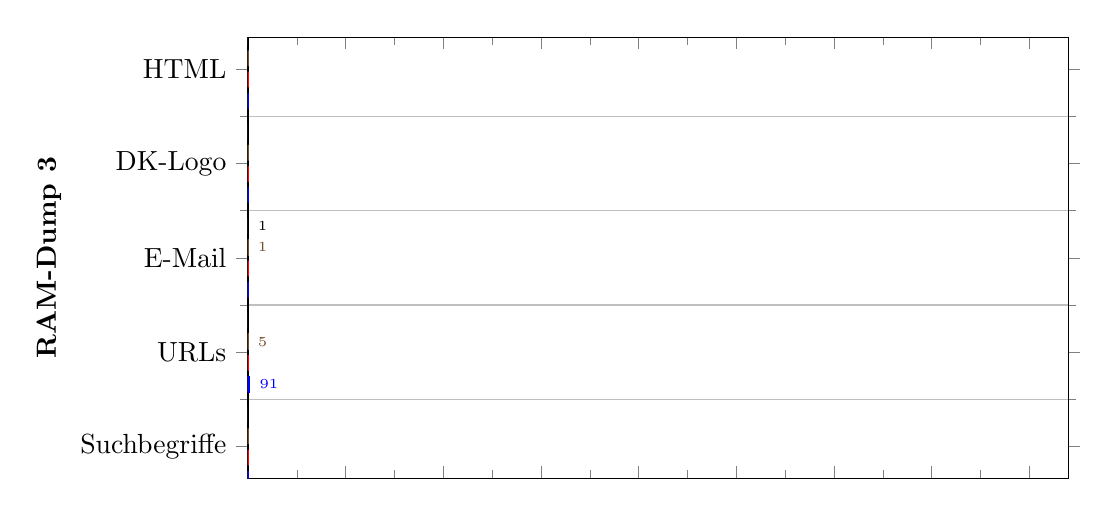
\begin{tikzpicture}
			\begin{axis}[
			xbar,
			width=12cm, 
			height=3cm, 
			ylabel style={align=center}, ylabel=\textbf{RAM-Dump 3},
			y=1.2cm,
			symbolic y coords={Suchbegriffe, URLs, E-Mail, DK-Logo, HTML},
			ytick=data,
			xticklabels={,,},
            xmin = 0,
            xmax = 42000,
			nodes near coords, 
			nodes near coords align={horizontal},
			nodes near coords style={font=\tiny},
   			nodes near coords={\pgfmathfloatifflags{\pgfplotspointmeta}{0}{}{\pgfmathprintnumber{\pgfplotspointmeta}}},
			bar width=.2cm,
			enlarge y limits={abs=2*\pgfplotbarwidth},
			scaled x ticks=false,
    		yminorgrids = true,minor tick num=1,
			legend style={
				at={(0.5,-0.1)},
				anchor=north
			},
			legend columns=4
			]
				\addplot coordinates {
				(0,Suchbegriffe) (91,URLs) (0,E-Mail) (0,DK-Logo) (0,HTML)
				};
				\addplot coordinates {
				(0,Suchbegriffe) (0,URLs) (0,E-Mail) (0,DK-Logo) (0,HTML)
				};
				\addplot coordinates {
				(0,Suchbegriffe) (5,URLs) (1,E-Mail) (0,DK-Logo) (0,HTML)
				};
				\addplot coordinates {
				(0,Suchbegriffe) (0,URLs) (1,E-Mail) (0,DK-Logo) (0,HTML)
				};
			\end{axis}
%			\legend{Firefox, Tor, Chrome, Brave}
		\end{tikzpicture}
		\\[-7pt]
		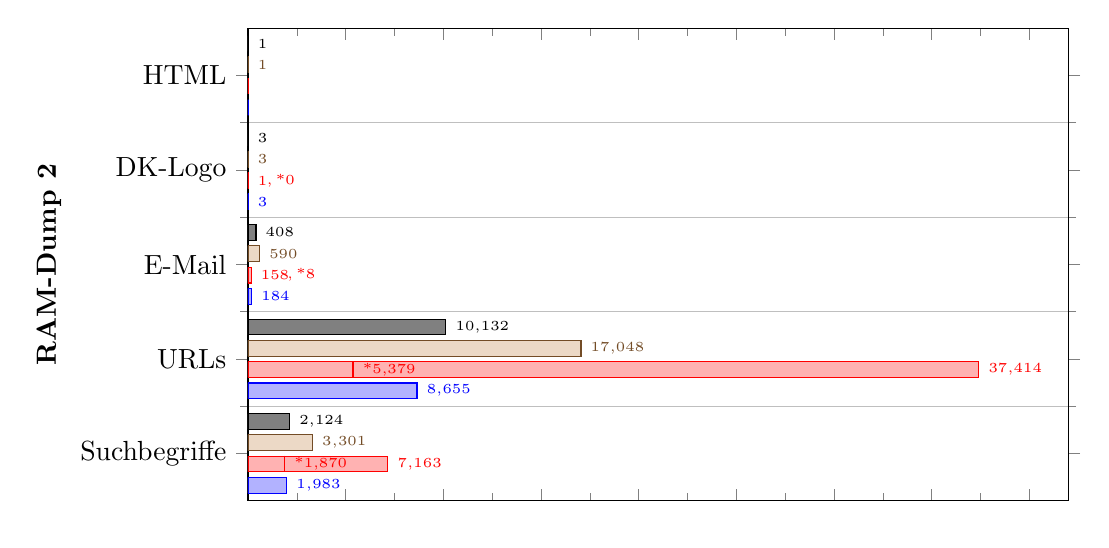
\begin{tikzpicture}
			\begin{axis}[
			xbar,
			width=12cm, 
			height=3cm, 
			ylabel style={align=center}, ylabel=\textbf{RAM-Dump 2},
			y=1.2cm,
%			symbolic y coords={Suchbegriffe, URLs, E-Mail, DK-Logo},
			ytick = {1,...,5},
			yticklabels={Suchbegriffe, URLs, E-Mail, DK-Logo, HTML},
			ytick=data,
			xticklabels={,,},
            xmin = 0,
            xmax = 42000,
			nodes near coords, 
			nodes near coords align={horizontal},
			nodes near coords style={font=\tiny},
   			nodes near coords={\pgfmathfloatifflags{\pgfplotspointmeta}{0}{}{\pgfmathprintnumber{\pgfplotspointmeta}}},
			bar width=.2cm,
			enlarge y limits={abs=3*\pgfplotbarwidth},
			scaled x ticks=false,
    		yminorgrids = true,minor tick num=1,
			legend style={
				at={(0.5,-0.1)},
				anchor=north
			},
			legend columns=4
			]
				\path  [red,line width=0pt] (axis cs: 500,3.977) -- (axis cs: 500,3.8)
				node[pos = 0.5,right] {\tiny,$\,$*0};
				\addplot coordinates {
				(1983,1) (8655,2) (184,3) (3,4) (0,5)
				};
				\path  [red,line width=0pt] (axis cs: 1550,2.977) -- (axis cs: 1550,2.8)
				node[pos = 0.5,right] {\tiny,$\,$*8};
				\addplot coordinates {
				(7163,1) (37414,2) (158,3) (1,4) (0,5)
				};
				\draw [red,line width=0.5pt] (axis cs: 5379,1.977) -- (axis cs: 5379,1.8)
				node[pos = 0.5,right] {\tiny*5,379};
				\addplot coordinates {
				(3301,1) (17048,2) (590,3) (3,4) (1,5)
				};
				\draw [red,line width=0.5pt] (axis cs: 1870,0.977) -- (axis cs: 1870,0.8)
				node[pos = 0.5,right] {\tiny*1,870};
				\addplot coordinates {
				(2124,1) (10132,2) (408,3) (3,4) (1,5)
				};
			\end{axis}
%			\legend{Firefox, Tor, Chrome, Brave}
		\end{tikzpicture}
		\\[-7pt]
		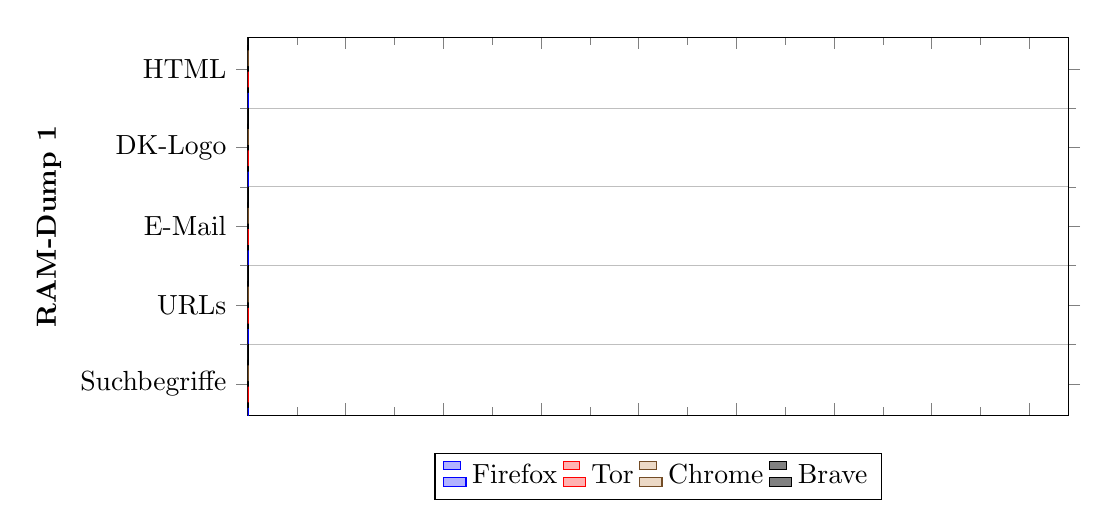
\begin{tikzpicture}
			\begin{axis}[
			xbar,
			width=12cm, 
			height=3cm, 
			ylabel style={align=center}, ylabel=\textbf{RAM-Dump 1},
			y=1cm,
%			symbolic y coords={Suchbegriffe, URLs, E-Mail, DK-Logo},
			ytick = {1,...,5},
			yticklabels={Suchbegriffe, URLs, E-Mail, DK-Logo, HTML},
%			ytick=data,
			xticklabels={,,},
            xmin = 0,
            xmax = 42000,
			nodes near coords, 
			nodes near coords align={horizontal},
			nodes near coords style={font=\tiny},
   			nodes near coords={\pgfmathfloatifflags{\pgfplotspointmeta}{0}{}{\pgfmathprintnumber{\pgfplotspointmeta}}},
			bar width=.2cm,
			enlarge y limits={abs=2*\pgfplotbarwidth},
			scaled x ticks=false,
    		yminorgrids = true,minor tick num=1,
			legend style={
				at={(0.5,-0.1)},
				anchor=north
			},
			legend columns=4
			]
				\addplot coordinates {
				(0,1) (0,2) (0,3) (0,4) (0,5)
				};
				\addplot coordinates {
				(0,1) (0,2) (0,3) (0,4) (0,5)
				};
				\addplot coordinates {
				(0,1) (0,2) (0,3) (0,4) (0,5)
				};
				\addplot coordinates {
				(0,1) (0,2) (0,3) (0,4) (0,5)
				};
			\legend{Firefox, Tor, Chrome, Brave}
			\end{axis}
		\end{tikzpicture}	
	\end{tabular}
	}
	\caption{Zusammenfassung gefundener Artefakte im RAM der Browser}
	\label{chart:all-browsers-ram-summary}
\end{table}

\paragraph*{Firefox vs Tor}
%> RAM-Dump 2: 
Tor hinterlässt nach dem Browsing Szenario, vor Zuweisung einer ``Neuen Identität`` mehr URL-Artefake und Suchbegriffe im RAM als Firefox (RAM-Dump 2). 
Sowohl bei Tor als auch bei Firefox ist zu diesem Zeitpunkt das Gmail-Passwort als Klartext im RAM identifizierbar.
Wie anhand der roten, mit * gekennzeichneten Werte in Abbildung \ref{chart:all-browsers-ram-summary} zu erkennen ist, 
reduzieren sich reduziert sich die hinterlassenen Artefakte nach Zuweisung einer ``Neuer Identität`` für den Tor-Browsers deutlich, sodass danach weniger Artefakte als bei Firefox vorhanden sind.
Wie in Kapitel \ref{section:methodik-vorbereitung-browserauswahl} erklärt, ermöglicht die ``Neue Identität`` ermöglicht das Schließen von Tabs und Fenstern, das Löschen von privaten Informationen und die Neukonfiguration der Tor-Netzwerkverbindung.
Mit der ``Neue Identität`` ist bei Tor das Passwort nicht mehr als Klartext im Arbeitsspeicher zu identifizieren.
%> RAM-Dump 3:
Nach Schließen des Browsers (RAM-Dump 3) hinterlässt der Tor Browser keine Artefakte, bei Firefox konnten noch 91 URLs im DNSCache gefunden werden. 
Keiner der beiden Browser hinterließ zu einem Zeitpunkt HTML-Artefakte.
%Gewinner:
%> RAM-Dump 2:
%	- Vor ``Neue Identität``: Firefox
%	- Nach ``Neuer Identität``: Tor 
%> RAM-Dump 3:
%	- Tor 
%Somit hinterlässt Tor sowohl nach dem Browsing Szenario mit ``Neuer Identität`` als auch mit geschlossenem Browser weniger PB Artefakte als Firefox.

\paragraph*{Chrome vs Brave}
*** TODO: Christoph ***\\
(Brave hinterlässt weniger Artefakte als Chrome)

\paragraph*{Firefox vs Chrome}
%> In RAM-Dump 2: 
Firefox hinterlässt nach dem Browsing Szenario mit geöffnetem Browser (RAM-Dump 2) in jeder Kategorie gleich viele (DK-Logo) oder weniger (E-Mail, URLs, Suchbegriffe, HTML) Artefakte als Chrome.
Dabei werden bei Firefox im zweiten RAM-Dump durchschnittlich 2.024 Artefakte weniger gefunden als bei Chrome.
%> In Ram-Dump 3: 
Nach Schließen des Browsers (RAM Dump 3) hinterlässt Firefox mehr URLs im Arbeitsspeicher als Chrome. Im RAM-Dump von Chrome wurde zusätzlich die Absender-Adresse gefunden.
%Gewinner:
%RAM-Dump 2:
%	- Firefox
%RAM-Dump 3: 
%	- URLs: Chrome
%	- E-Mail: Firefox

\paragraph*{Tor vs Brave}
Vor Zuweisung der ``Neuen Identität`` hinterlässt der Tor-Browser nach dem Browsing-Szenario  deutlich mehr URL- und Suchbegriff-Artefakte als Brave (RAM-Dump 2). Insbesondere hinterlässt Tor zweimal das Passwort des Google-Accounts als Klartext im RAM.
Nach Zuweisung der ``Neuen Identiät`` des Tor-Browsers hinterlässt dieser durchschnittlich 1315 Artefakte weniger als Brave.
Nach Schließen des Browsers (RAM-Dump 3) hinterlässt Tor kein Artefakt im RAM, Brave einmal die Absender-Mail. 
%Gewinner:
%RAM-Dump 2:
%	- DK-Logo, E-Mail: Tor
%	- URLs, Suchbegriffe: Brave (Vor ``Neue Identität``), Tor (Nach ``Neuer Identität``) 
%RAM-Dump 3: Tor

\paragraph*{Quantitativer Vergleich aller Browser}
Um unter den vier untersuchten Browsern denjenigen mit den wenigsten PB Artefakten zu ermitteln, wird eine in Tabelle \ref{tab:gewinner-tabelle} gezeigte, sogenannte  \textit{Gewinner-Tabelle} erstellt \cite{Horsman.2019}.

\begin{table}[h!]
	\caption{Gewinner-Tabelle der vier untersuchten Browser}
	\label{tab:gewinner-tabelle}
	\centering
	\resizebox{\linewidth}{!}{
	\begin{tabular}{c|c|c|c|c|c|c}
	\cline{2-7}
	\multicolumn{1}{l|}{}                                                                                                & \textbf{Suchbegriffe}                   & \textbf{URLs}                                                                                     & \textbf{E-Mail}                                                                                    & \textbf{DK-Logo}                    & \textbf{HTML}                                                                           & \multicolumn{1}{c|}{\textbf{\begin{tabular}[c]{@{}c@{}}Gewinner \\ pro RAM-Dump\end{tabular}}} \\ \hline
	\multicolumn{1}{|c|}{\textbf{RAM-Dump 1}}                                                                            & Unentschieden                           & Unentschieden                                                                                     & Unentschieden                                                                                      & Unentschieden                       & Unentschieden                                                                           & \multicolumn{1}{c|}{{\color[HTML]{FE0000} \textbf{Unentschieden}}}                             \\ \hline
	\multicolumn{1}{|c|}{\textbf{\begin{tabular}[c]{@{}c@{}}RAM-Dump 2\\ (ohne "Neuer ID")\end{tabular}}}                & Firefox                                 & Firefox                                                                                           & Brave*                                                                                             & Tor                                 & \begin{tabular}[c]{@{}c@{}}Firefox, \\ Tor\end{tabular}                                 & \multicolumn{1}{c|}{{\color[HTML]{FE0000} \textbf{Firefox}}}                                   \\ \hline
	\multicolumn{1}{|c|}{\textbf{\begin{tabular}[c]{@{}c@{}}RAM-Dump 2\\ (mit "Neuer ID")\end{tabular}}}                 & Tor                                     & Tor                                                                                               & Tor                                                                                                & Tor                                 & \begin{tabular}[c]{@{}c@{}}Firefox, \\ Tor\end{tabular}                                 & \multicolumn{1}{c|}{{\color[HTML]{FE0000} \textbf{Tor}}}                                       \\ \hline
	\multicolumn{1}{|c|}{\textbf{RAM-Dump 3}}                                                                            & Unentschieden                           & Tor, Brave                                                                                        & \begin{tabular}[c]{@{}c@{}}Firefox, \\ Tor\end{tabular}                                            & Unentschieden                       & Unentschieden                                                                           & \multicolumn{1}{c|}{{\color[HTML]{FE0000} \textbf{Tor}}}                                       \\ \hline
	\multicolumn{1}{|c|}{\textbf{\begin{tabular}[c]{@{}c@{}}Gewinner pro \\ Kategorie\\ (ohne "Neuer ID")\end{tabular}}} & {\color[HTML]{FE0000} \textbf{Firefox}} & {\color[HTML]{FE0000} \textbf{\begin{tabular}[c]{@{}c@{}}Firefox, \\ Tor, \\ Brave\end{tabular}}} & {\color[HTML]{FE0000} \textbf{\begin{tabular}[c]{@{}c@{}}Firefox, \\ Tor, \\ Brave*\end{tabular}}} & {\color[HTML]{FE0000} \textbf{Tor}} & {\color[HTML]{FE0000} \textbf{\begin{tabular}[c]{@{}c@{}}Firefox, \\ Tor\end{tabular}}} & \multicolumn{1}{l}{}                                                                           \\ \cline{1-6}
	\multicolumn{1}{|c|}{\textbf{\begin{tabular}[c]{@{}c@{}}Gewinner pro \\ Kategorie\\ (mit "Neuer ID")\end{tabular}}}  & {\color[HTML]{FE0000} \textbf{Tor}}     & {\color[HTML]{FE0000} \textbf{Tor}}                                                               & {\color[HTML]{FE0000} \textbf{Tor}}                                                                & {\color[HTML]{FE0000} \textbf{Tor}} & {\color[HTML]{FE0000} \textbf{\begin{tabular}[c]{@{}c@{}}Firefox, \\ Tor\end{tabular}}} & \multicolumn{1}{l}{}                                                                           \\ \cline{1-6}
	\end{tabular}
	}
\end{table}

Dabei liegt der Fokus auf den Kategorien der PB-Artefakte:  Es wird für jede RAM-Dump/Kategorie Kombination derjenige Browser mit den wenigsten PB Artefakten ermittelt. 
Somit wird die Anzahl gefundener Artefakte wird nur innerhalb einer Kategorie verglichen. Die Differenz gefundener PB Artefakte wird dabei nicht berücksichtigt.
Per Mehrheitseinscheid ergeben sich daraus zwei Arten von \textit{Gewinnern}:
\begin{itemize}
\item \textbf{Gewinner pro RAM-Dump}: Browser, der innerhalb eines RAM-Dumps am häufigsten die wenigsten PB Artefakte einer Kategorie hinterlässt. (Zeilenweiser Mehrheitsentscheid)
\item \textbf{Gewinner pro Kategorie}: Browser, der innerhalb einer Kategorie am häufigsten die wenigsten PB-Artefakte in den RAM-Dumps hinterlässt. (Spaltenweiser Mehrheitsentscheid)
\end{itemize}

Um ein differenziertes Ergebnis zu ermitteln, wird bei RAM-Dump 2 zusätzlich unterschieden, ob der Tor-Browser vor- oder nach der Zuweisung der ``Neuen Identität``, kurz ``Neue ID``, bewertet wird. 
Diese Unterscheidung findet ebenfalls bei den Gewinnern statt. Somit ergeben sich die in Tabelle \ref{tab:gewinner} ermittelten vier Gewinner:

\begin{table}[h!]
	\centering
	\caption{Ermittelte Gewinner gemäß Gewinner-Tabelle}
	\label{tab:gewinner}
	\resizebox{0.8\linewidth}{!}{
	\begin{tabular}{c|c|c|}
	\cline{2-3}
	\multicolumn{1}{l|}{}                                 & \textbf{Mit ``Neuer Identität``} & \textbf{Ohne ``Neuer Identität``} \\ \hline
	\multicolumn{1}{|c|}{\textbf{Gewinner pro RAM-Dump}}  & Tor                            & Firefox, Tor                    \\ \hline
	\multicolumn{1}{|c|}{\textbf{Gewinner pro Kategorie}} & Tor                            & Firefox, Tor                    \\ \hline
	\end{tabular}
	}
\end{table}

Unter Berücksichtigung der ``Neuen Identität`` ist der Tor-Browser sowohl der Gewinner pro RAM-Dump als auch pro Kategorie.
Ohne Berücksichtigung ist neben dem Tor-Browser auch Firefox Gewinner pro RAM-Dump und pro Kategorie. Somit ist gemäß Auswertung der Gewinner-Tabelle der Tor-Browser derjenige Browser mit den wenigsten PB Artefakten, gefolgt von Mozilla Firefox.











